\section{Architecture}
\label{sec:Architecture}

\subsection{Architecture model}
The WOMBAT application depends on the Launcher project and Oasis project, but WOMBAT is designed to function as an independent application with minor modifications to cooperate with the GIRAF launcher and Oasis.
We choose to design WOMBAT as an independent application, because it was easier to modify features in the application when they were ready, instead of waiting for the features to be implemented in the GIRAF Launcher or Oasis. 
The dependency diagram of the WOMBAT architecture can be found in \autoref{fig:WombatDependency}.
The WOMBAT architecture is a five layer architecture which enhances how you can perform testing and do collaborative work. 
The five layers consists of: 

\begin{itemize}
	\item[Main] \hfill \\	This layer is the main activity of WOMBAT which means that it initiate the whole WOMBAT application. The main layer is dependent on the Tools layer since it contains the initiating tools. 
	\item [Layout] \hfill \\	This layer consists of the three fragments; profile fragment, configuration fragment, and customize fragment, and the custom \texttt{ArrayAdapter}s which WOMBAT uses. The layout layer is depended on the Tools layer since it contains the objects and methods that is required for the layout to work. The Layout layer is also depended on the Main layer, without the Main layer the Layout layer would never be initiated. The Layout layer is depended on the Draw layer, the Draw layer delivers the methods that generates the \texttt{View}s for the timers and pictograms.
	\item [Draw] \hfill \\	The Draw layer contains the methods that generate the \texttt{View}s of the timers and pictograms. Draw layer is depended on the Tools layer since the Tools layers contain all the different types of objects that the Draw layer implements. The Draw layer is also depended on the Layout layer, the Layout layer initiate the Draw layer.
	\item [Tools] \hfill \\	This layer consists of all the types of objects and methods that WOMBAT uses. The Tools layer is depended on the Main layer to initiate the proper objects, you can read more about this in section: \ref{subsec:TimerLib}. The Tools layer is also depended on the CRUD layer which contains the connection to the \texttt{OasisLocalDatabase}.
	\item [CRUD] \hfill \\	This layer is responsible for saving and loading from the \texttt{OasisLocalDatabase}, it is depended on the Tools layer because it uses the objects and methods that the Tools layer provides.
\end{itemize}

\begin{figure}[H]
	\centering
		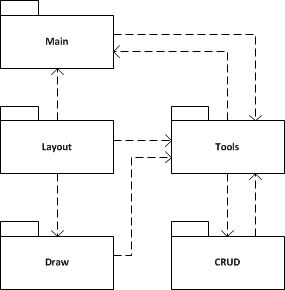
\includegraphics[scale=0.6]{Images/Implementation/WombatDependency.png}
	\caption{Dependecy diagram of WOMBAT architecture}
	\label{fig:WombatDependency}
\end{figure}

\subsubsection{Library}

The original idea was to split the layers into two projects, that way it would be able to conduct tests outside the main layer. The first project would be an Android project with a main activity, WOMBAT. The second project would be an Android library which should contain all the back-end functionality, \texttt{TimerLib}. This is how the two projects would look like:

\begin{description}
  \item[WOMBAT] \hfill \\\begin{itemize}  \item Main layer  \item Layout layer
\end{itemize}
  \item[TimerLib] \hfill \\\begin{itemize}  \item Tools layer  \item Draw layer  \item CRUD layer
\end{itemize}
\end{description}

We later decided to redesign, and make three projects instead of two projects. We choose the redesign because that we are three developers in our project whom all want to conduct independent testing. The first project, WOMBAT, will stay as it originally was. The Second project is split into two projects, \texttt{TimerLib} and \textt{DrawLib}. \texttt{TimerLib} contains the Tools layer and the CRUD layer. The \texttt{DrawLib} contains the draw layer.

\begin{description}
  \item[WOMBAT] \hfill \\\begin{itemize}  \item Main layer  \item Layout layer\end{itemize}
  \item[TimerLib] \hfill \\\begin{itemize}  \item Tools layer  \item CRUD layer
\end{itemize}
  \item[DrawLib] \hfill \\\begin{itemize}  \item Draw layer\end{itemize}
\end{description}

The dependency diagram of the WOMBAT projects can be found in figure \ref{fig:LibraryDependency}.

\begin{figure}[H]
	\centering
		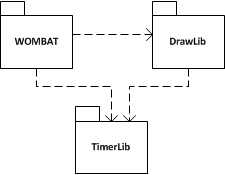
\includegraphics[scale=0.6]{Images/Implementation/LibraryDependency.png}
	\caption{Dependecy diagram of WOMBAT projects}
	\label{fig:LibraryDependency}
\end{figure}

\subsubsection{Wombat lifecycle}
You can see a detailed flowchart over the WOMBAT life cycle on figure \ref{fig:wombatLifeCycle}. The flowchart describes whatever that can occur while the WOMBAT application is running. The flowchart can help debug and understand the application if somebody chooses to develop further on WOMBAT.

\begin{figure}[H]
	\centering
		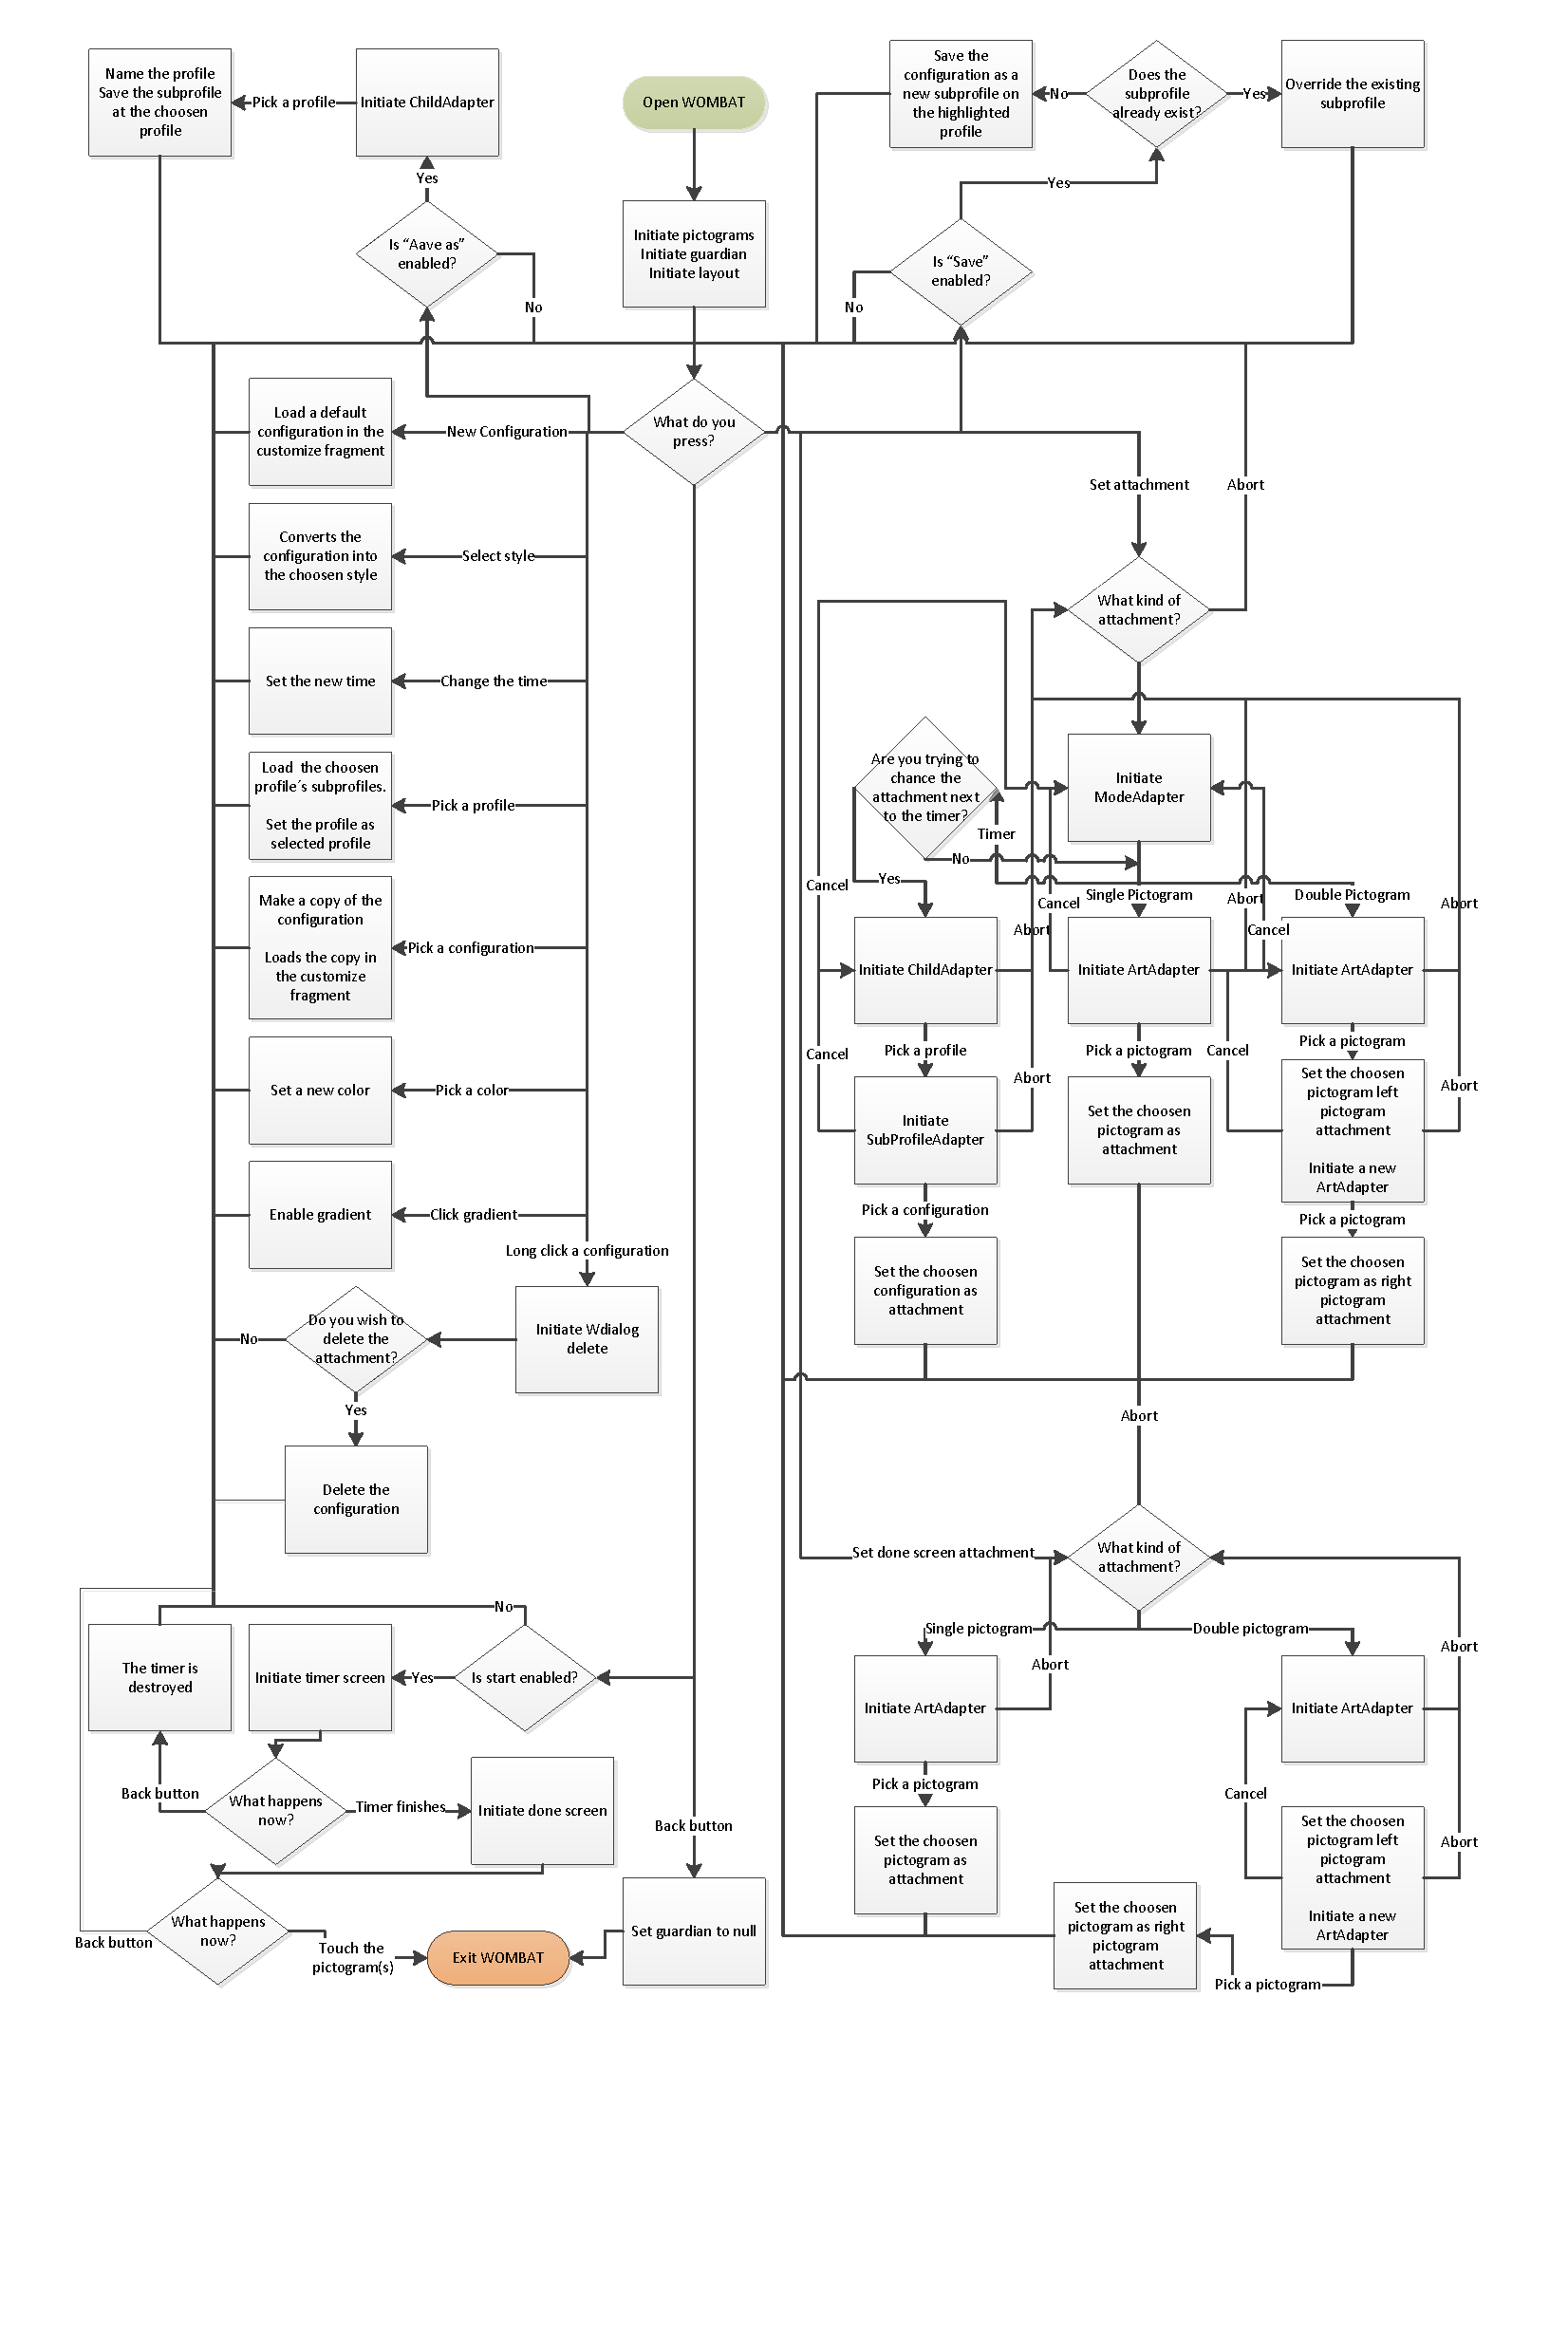
\includegraphics[scale=0.6]{Images/Implementation/wombatLifeCycle.pdf}
	\caption{Flowchart of WOMBAT lifecycle}
	\label{fig:wombatLifeCycle}
\end{figure}